\documentclass[9pt]{amsart}
\usepackage[letterpaper, left=.5in, right=.5in, top=.5in, bottom=.5in]{geometry}
\usepackage{amscd,amssymb}
\usepackage{kpfonts}
\usepackage{xcolor}
\usepackage{listings}
\usepackage{graphicx}
 
\usepackage{multicol}

\setlength{\parindent}{0pt}
\setlength{\parskip}{1pt}
\renewcommand{\baselinestretch}{1.3}

\lstset{basicstyle=\footnotesize}

\setlength{\columnseprule}{.1pt}
\setlength{\columnsep}{10pt}
\def\columnseprulecolor{\color{black}}

 
\begin{document}
\begin{multicols*}{3}
  [
    \textbf{Final Cheat Sheet - CS 4150}
  ]

  \textbf{Complexity Analysis}
  \newline
  $f(n) < g(n) \Rightarrow f(n)\ \text{is}\ o(g(n))$
  \newline 
  $f(n) \leq g(n) \Rightarrow f(n)\ \text{is}\ O(g(n))$
  \newline
  $f(n) = g(n) \Rightarrow f(n)\ \text{is}\ \theta(g(n))$
  \newline
  $f(n) \geq g(n) \Rightarrow f(n)\ \text{is}\ \Omega(g(n))$
  \newline
  $f(n) > g(n) \Rightarrow f(n)\ \text{is}\ \omega(g(n))$
  \vskip 5pt
  $f(n)\ \text{is}\ O(g(n))$ if $\exists c, n_0 > 0$ such that
  $0 \leq f(n) \leq cg(n)$, $\forall n \geq n_0$.

  \vskip 5pt

  Note: \\
  $f$ could be $O(n^2)$ and $g$ could be $O(n^3)$ but $f$ is not $O(g)$ because $f$ could be $n^2$ and $g$ could be $n$. If $g$ was instead $\omega(n^3)$, then $f$ is $O(g)$.
  
  \vskip 7pt
  \hrule
  \vskip 7pt

  \textbf{Domination Order}
  \footnotesize
  \begin{center}
  \begin{tabular}{c | c | c}
     \emph{f(n)} & \emph{restriction} & \emph{when $a > b$} \\
     \hline
     $n! \text{ / } n^n$ & & \\
     \hline
     $a^n$ & $a > 1$ & $a^n > b^n$ \\
     \hline
     $n^a$ & $a > 0$ & $n^a > n^b$ \\
     \hline
     $(\log(n))^a$ & $a > 0$ & $(\log(n))^a > (\log(n))^b$ \\
     \hline
     1 & &
  \end{tabular}
  \end{center}
  \normalsize
  Separate terms and compare with domination table ($n \log(n)$ vs $n^2 \log(n)$, $n^2$ 
  dominates and $\log(n)$ are tied so the latter dominates.)

  \vskip 7pt
  \hrule
  \vskip 7pt

  \textbf{Doubling Behavior}
  \footnotesize
  \begin{center}
  \begin{tabular}{c | c | c}
     \emph{f(n)} & \emph{name} & \emph{doubling behavior} \\
     \hline
     1 & constant & stays the same \\
     \hline
     log(n) & log & incr by const \\
     \hline
     n & linear & doubles \\
     \hline
     nlog(n) & n log n & $>$double \\
     \hline
     $n^2$ & quadratic & quadruples \\
     \hline
     $n^3$ & cubic & octuples \\
     \hline
     $2^n$ & exponential & squares
  \end{tabular}
  \end{center}
  \normalsize

  \vskip 7pt
  \hrule
  \vskip 7pt
  
  \textbf{Master Theorem}
  \newline
  If $T(n) = aT(n/b) + O(n^d)$ for constants $a > 0, b > 1, d \geq 0$, then:
  $$
  T(n) = 
  \begin{cases}
    O(n^d) & \text{if } d > \log_b(a) \\
    O(n^d \log(n)) & \text{if } d = \log_b(a) \\
    O(n^{\log_b(a)}) & \text{if } d < \log_b(a)
  \end{cases}
  $$

  \vskip 7pt
  \hrule
  \vskip 7pt

  \textbf{Summations}
  $$
  \sum^n_{i=1} i = \frac{n(n+1)}{2}
  $$
  For $r \neq 1$:
  $$
  \sum^{n-1}_{k=0} ar^k = a(\frac{1 - r^n}{1 - r})
  $$

  \textbf{Exponents}
  $$a^n * a^m = a^{n+m}$$
  $$a^n * b^n = (a * b)^n$$
  $$a^n / a^m = a^{n-m}$$
  $$a^n * b^n = (a / b)^n$$
  $$(b^n)^m = b^{n*m}$$
  $$b^{n^m} = b^{(n^m)}$$

  \vskip 7pt
  \hrule
  \vskip 7pt

  \textbf{Logarithms}
  $$\log_b(M * N) = \log_b M + \log_b N$$
  $$\log_b(\frac{M}{N}) = \log_b M - \log_b N$$
  $$\log_b(M^k) = k * \log_b M$$
  $$\log_b(1) = 0$$
  $$\log_b(b) = 1$$
  $$\log_b(b^k) = k$$
  $$b^{\log_b(k)} = k$$
  $$\log(n!) \approx \log(n^n) = n\log(n)$$

  \vskip 7pt
  \hrule
  \vskip 7pt

  \textbf{Modular Arithmetic}
  \newline
  $x \mod N = x + kN$ where $k \in \mathbb{Z}$ and $0 \leq x + kN < N$.
  \vskip 3pt
  For $x \geq 0$, $x \mod N$ is the remainder after dividing by $N$. For $x < 0$,
  $x \mod N$ is $N - (-x \mod N)$.
  \vskip 3pt
  $a \equiv b (\text{mod } n)$ means that $a$ and $b$ are equivalent in 
  $(\text{mod } n)$.
  \vskip 3pt
  If $x \equiv x' \mod N$ and $y \equiv y' \mod N$, then
  $$x + y \equiv x' + y' \mod N$$
  $$xy \equiv x'y' \mod N$$
  $$x^y \equiv (x')^y \mod N$$
  $$x^y \not\equiv (x')^{y'} \mod N$$ 
  Exponent example:
  $$3^{100} \mod 26 \Rightarrow 3(3^3)^{33} \mod 26 \Rightarrow$$
  $$(3 \mod 26)(27 \mod 26)^{33} \Rightarrow 3 * 1^{33} = 3$$
  $x$ is the multiplicative inverse if
  $$ax \equiv 1 \mod N$$
  Example:
  $$9^{-1} \mod 11 = 5$$
  $$3^{-1} \mod 13 \Rightarrow 3x + 13y = 1 \Rightarrow$$
  $$x = -4, y = 1 \Rightarrow -4 \equiv 9 \mod 13$$
  Therefore $3^{-1} \mod 13 = 9$.

  \textbf{Modular Arithmetic Cont.}
  \newline
  Modular addition is $O(n)$ and modular multiplication is $O(n^2)$, where $n$ is the
  length of the modulus (in $log(N)$ for base 2). 
  \newline
  For exponentiation, split $x^8$ to
  $((x^2)^2)^2)$ then take the mod at each exponentiation 
  \newline
  Example when $x = 4$: 
  $$4^2 \mod 7 = 2 \Rightarrow 2^2 \mod 7 = 4 \Rightarrow$$
  $$4^2 \mod 7 = 2 \Rightarrow 2 \equiv 4^8 \mod 7$$

  \vskip 7pt
  \hrule
  \vskip 7pt

  \textbf{Greatest Common Divisor}
  \begin{lstlisting}
    gcd(a, b)
      while (b > 0)
        aModB = a mod B
        a = b
        b = aModB
      return a
  \end{lstlisting}

  \vskip 7pt
  \hrule
  \vskip 7pt

  \textbf{Sets and Maps}
  \newline
  With balanced binary search tree (worst cases become $\Theta(n)$ with no balance):
  \footnotesize
  \begin{center}
  \begin{tabular}{c | c | c}
     \emph{operation} & \emph{best case} & \emph{worst case} \\
     \hline
     Insert & $\Theta(\log n)$ & $\Theta(\log n)$ \\
     \hline
     Remove & $\Theta(\log n)$ & $\Theta(\log n)$ \\
     \hline
     Lookup & $\Theta(1)$ & $\Theta(\log n)$ \\
     \hline
     Iterate & $\Theta(n)$ & $\Theta(n)$ \\
  \end{tabular}
  \end{center}
  \normalsize

  With Hash Table (worst cases become $\Theta(n)$ with bad hash):
  \footnotesize
  \begin{center}
  \begin{tabular}{c | c | c}
     \emph{operation} & \emph{best case} & \emph{worst case} \\
     \hline
     Insert & $\Theta(1)$ & $\Theta(1)$ \\
     \hline
     Remove & $\Theta(1)$ & $\Theta(1)$ \\
     \hline
     Lookup & $\Theta(1)$ & $\Theta(1)$ \\
     \hline
     Iterate & $\Theta(n)$ & $\Theta(n)$ \\
  \end{tabular}
  \end{center}
  \normalsize

  \vskip 7pt
  \hrule
  \vskip 7pt

  \textbf{Dynamic Arrays}
  \newline
  Dynamic array is better at random access.
  \footnotesize
  \begin{center}
  \begin{tabular}{c | c | c}
     \emph{operation} & \emph{best case} & \emph{worst case} \\
     \hline
     Get & $\Theta(1)$ & $\Theta(1)$ \\
     \hline
     AddLast & $\Theta(1)$ & $\Theta(n)$ \\
     \hline
     $k$ AddLasts & $\Theta(k)$ & $\Theta(k)$ \\
     \hline
     Iterate & $\Theta(n)$ & $\Theta(n)$ \\
     \hline
     GetAt & $\Theta(1)$ & $\Theta(1)$ \\
     \hline
     AddAt & $\Theta(1)$ & $\Theta(n)$ \\
     \hline
     Remove & $O(1)$ & $O(n)$
  \end{tabular}
  \end{center}
  \normalsize

  \vskip 7pt
  \hrule
  \vskip 7pt

  \textbf{Linked Lists}
  \newline
  Linked lists are better for insertion.
  \footnotesize
  \begin{center}
  \begin{tabular}{c | c | c}
     \emph{operation} & \emph{best case} & \emph{worst case} \\
     \hline
     Get & $\Theta(1)$ & $\Theta(n)$ \\
     \hline
     AddLast & $\Theta(1)$ & $\Theta(1)$ \\
     \hline
     Iterate & $\Theta(n)$ & $\Theta(n)$ \\
     \hline
     GetAt & $\Theta(1)$ & $\Theta(1)$ \\
     \hline
     AddAt & $\Theta(1)$ & $\Theta(1)$ \\
  \end{tabular}
  \end{center}
  \normalsize

  \columnbreak
  \textbf{Amortized Analysis}
  \footnotesize
  \begin{center}
  \begin{tabular}{c | c | c}
     \emph{operation} & \emph{ending size} & \emph{cost} \\
     \hline
     1 AddLast & 1 & a \\
     Resize & & r \\
     \hline
     1 AddLast & 2 & a \\
     Resize & & 2r \\
     \hline
     2 AddLasts & 4 & 2a \\
     Resize & & 4r \\
     \hline
     4 AddLasts & 8 & 4a \\
     Resize & & 8r \\
     \hline
     $2^k$ AddLasts & $2^{k+1}$ & $2^k$a \\
     Resize & & $2^{k+1}$r
  \end{tabular}
  \end{center}
  \normalsize
  Sum the AddLast costs to get $2^{k+1}a$. Sum the Resize costs to get $(2^{k+2}-1)r$.
  Add these together to get the total cost of $2^{k+1}(a+2r) - r$. Divide by the number 
  of AddLasts performed $2^{k+1}$. Average cost is then $\frac{a+2r - r}{2^{k+1}}$
  (constant time).

  \vskip 7pt
  \hrule
  \vskip 7pt

  \textbf{Algorithms}
  \newline
  Unordered arrays will always take $\Theta(n)$ time to search, equivalent to linear search.
  \newline
  Ordered arrays can use binary search, which takes $O(\log n)$ time.
  \footnotesize
  \begin{center}
  \begin{tabular}{c | c | c | c}
     \emph{sort} & \emph{best case} & \emph{worst case} & \emph{stable} \\
     \hline
     Selection & $O(n^2)$ & $O(n^2)$ & no \\
     \hline
     Insertion & $O(n)$ & $O(n^2)$ & yes \\
     \hline
     Merge & $O(n \log n)$ & $O(n \log n)$ & yes \\
     \hline
     Quick & $O(n \log n)$ & $O(n^2)$ & no \\
  \end{tabular}
  \end{center}
  \normalsize
  Selection will go through each index and search the rest of the list for what should be
  in that index. Insertion will go through each value and move it as far left as it can go.
  Merge sort recursively splits then merges lists in order. Quicksort uses a pivot where
  everything to the left of the pivot will be less than the value of the pivot.
  \vskip 5pt
  Sorting lower bound is $\Omega(n \log n)$ due to the decision tree of all possible sorting
  outcomes.

  \vskip 7pt
  \hrule
  \vskip 7pt

  \textbf{Karatsuba Multiplication}
  \newline
  Split $x$ and $y$ into $(x_L, y_L)$ and $(x_R, y_R)$.
  $$P_1 = x_L * y_L$$
  $$P_2 = x_R * y_R$$
  $$P_3 = x_L * y_L + x_L * y_R + x_R * y_L + x_R * y_R$$
  Return $P_1 * 2^n + (P_3 - P_1 - P_2) * 2^{n/2} + P_2$.
  \newline
  $T(n)$ is $O(n^{1.59})$. 
  \newline
  Standard recursive multiplication is:
  $$xy = (2^{n}x_L y_L + 2^{n/2}(x_L y_R + x_R y_L) + x_R y_R)$$
  which is $O(n^2)$. Do not use Karatsuba multiplication until the hardware can
  no longer handle the multiplication, creating a blended algorithm.
  
  \textbf{Selection}
  \newline
  To find the element that would be at $A[i]$ if $A$ was sorted, use an approach similar
  Quicksort with partitions. The best case would be $O(n)$ and the worst case is $O(n^2)$, significantly
  better than $O(n \log n)$ to sort.

  \vskip 7pt
  \hrule
  \vskip 7pt

  \textbf{Graph Representations}
  \footnotesize
  \begin{center}
  \begin{tabular}{r | c | c}
     & \emph{matrix} & \emph{adjacency list} \\
     \hline
     sparse space & $\Theta(V^2)$ & $\Theta(V)$ \\
     dense space & $\Theta(V^2)$ & $\Theta(V^2)$ \\
     edge from u to v & $\Theta(1)$ & $O(V)$, $O(E)$, $\Omega(1)$ \\
     edge out of u & $O(V)$, $\Omega(1)$ & $\Theta(1)$ \\
     all edges out of u & $\Theta(V)$ & $O(V)$, $O(E)$, $\Omega(1)$ \\
     all edges & $\Theta(V^2)$ & $\Theta(V+E)$ \\
  \end{tabular}
  \end{center}
  \normalsize

  \vskip 7pt
  \hrule
  \vskip 7pt

  \textbf{Depth First Search}
  \newline
  Used for topological sorting. Cost is $O(V) + O(E) + O(\text{ENUM ALL EDGES})$. 
  \newline
  Thus, $O(V + E)$ for adjacency list and $O(V^2)$ for matrix.
  \begin{center}
  \begin{tabular}{c | c}
  \begin{lstlisting}
dfs(g):
for each v in V
  visted[v] = false
for each v in V
  if !visited[v]
    explore(G, v)
  \end{lstlisting}
  &
  \begin{lstlisting}
explore(G, v):
visited[v] = true
previsit(v)
for each (v,u) in E
  if !visited[u]
    explore(G, u)
postvisit(v)
  \end{lstlisting}
  \end{tabular}
  \end{center}
  Order by descending post-visit numbers to get topological sort order (sources to sinks).
  There must be no cycles for topological sort.
  \footnotesize
  \begin{center}
  \begin{tabular}{c | c}
     \emph{pre/post comparisons} & \emph{edge type} \\
     \hline
     $\text{pre(u)} < \text{pre(v)} < \text{post(v)} < \text{post(u)}$ & child/forward \\
     \hline
     $\text{pre(v)} < \text{pre(u)} < \text{post(u)} < \text{post(v)}$ & parent/back \\
     \hline
     $(\text{pre(u)} < \text{post(u)}) \text{\&} (\text{pre(v)} < \text{post(v))}$ & cross \\
  \end{tabular}
  \end{center}
  \normalsize
  Depth first search will detect cycles if it finds a back edge.

  \vskip 7pt
  \hrule
  \vskip 7pt

  \textbf{Strongly Connected Components}
  \newline
  Topologically sort the vertices and iterate 
  through the sorted vertices. Look for cycles and remove vertices found in a cycle from 
  the list until no vertices are left.

  \vskip 7pt
  \hrule
  \vskip 7pt

  \textbf{Breadth-First Search} 
  \newline
  Used to find the shortest-path from one node to every other node in an unweighted, cyclic
  graph. Cost is $O(V) + O(E) + O(\text{ENUM})$. 
  \vskip 5pt
  Start from some vertex and add all of its edges to the queue, if vertex has not been
  visited yet. Continually pop from the 
  queue until it is empty. Update the prev/dist array as you pop from the queue.

  \vskip 20pt
  \textbf{Bellman-Ford}
  \newline
  Apply the `update` operation on all edges $V-1$ times or until a single iteration yields no
  changes. Assume no cycles of net negative cost, but negative weights are allowed.
  \newline
  Cost is $O(\text{V ENUM})$, which is $O(V^3)$ for a 
  matrix and $O(V^2 + VE)$ for an adjacency list.
  \begin{lstlisting}
update(u, v, w):
if dist[v] > dist[u] + w
    dist[v] = dist[u] + w
    prev[v] = u
  \end{lstlisting}
  If it is a DAG, we can topologically sort and go through all of the vertices once. The
  cost is then $O(\text{ENUM})$.

  \vskip 7pt
  \hrule
  \vskip 7pt

  \textbf{Dijkstra's Algorithm}
  \newline
  Finds the least-cost path in an cyclic graph with no negative edges. Follow the same
  algorithm as BFS, but use a priority queue where priority is determined by distance
  cost. Update vertices in the queue as cheaper paths are found.
  \newline Cost is 
  $O(\text{V DELETE}) + O(\text{E INSERT}) + O(\text{ENUM})  \Rightarrow O(V^2) \text{ or } O((E + V) \log V)$.
  
  \vskip 7pt
  \hrule
  \vskip 7pt

  \textbf{Priority Queue}
  \newline
  Priority queues can be represented as an unordered array where insert/update is $O(1)$ and
  delete is $O(V)$.
  \vskip 5pt
  A binary heap may also be used. For a binary heap, insertion is $O(\log n)$, delete
  is $O(\log n)$, and update can be made to be $O(1)$ with a hash map. To remove the
  root (A) from the binary heap, replace the element from the last-most spot (B) with the root.
  Delete A and then "bubble-down" B by continually swapping with the smallest child, 
  until it can no longer swap.
  \vskip 5pt
  Binary heaps allow for us to perform a heap-sort in $O(n \log n)$ time. Insertions
  and deletions cannot both be $O(1)$, as then heap-sort would become faster than
  $O(n \log n)$, violating the sorting lower bound.

  \vskip 7pt
  \hrule
  \vskip 7pt

  \textbf{Majority Element}
  \newline
  Iterate through the list. Replace leader when "wins" is equal to 0. Increase
  if leader wins against current. At the end, go through the list again and ensure that 
  leader element is the majority. The cost is $O(n)$.



\end{multicols*}
\pagebreak

\begin{multicols*}{3}
  \textbf{Greedy Algorithms} \\
  \textit{Optimal Substructure}: Every optimal solution contains within it optimal solutions to each of its subproblems.
  \vskip 2pt
  \textit{Overview}: At each stage, pick what is the best local option (ex: earliest ending time). Eliminate anything that is no longer a possibility. Repeat until finish.
  \vskip 2pt
  \textit{Correctness}: Every global optimal solution must contain the greedy choice at each local choice with the optimal substructure property. If it does not, then there must be another optimal solution with the greedy choice.

  \vskip 7pt
  \hrule
  \vskip 7pt

  \textbf{Minimum Spanning Tree} \\
  Always contains minimum weighted edge because of the cut property. \\
  \textit{Kruskal's Algorithm}: Repeatedly pick the lightest edge that does not create a cycle. Complexity is $O(\text{SORT}) + O(E * \text{FIND}) + O(V * \text{UNION}) \Rightarrow O(E \log(V)) \approx O(E)$.
  \vskip 2pt
  \textit{Prim's Algorithm}: Pick some starting vertex and let $S$ be a set that contains that starting vertex. Repeatedly pick the lightest edge that goes from a vertex in $S$ to a vertex not in $S$. Then add that vertex not in $S$ to $S$. Complexity is the same as Dijkstra's Algorithm.

  \vskip 7pt
  \hrule
  \vskip 7pt

  \textbf{Disjoint Sets} \\
  \textit{Creation}: Make $n$ singleton sets containing the integers $1$ to $n$.
  \vskip 2pt
  \textit{Find}: Returns the root element of the set.
  \vskip 2pt
  \textit{Union}: Combine two sets. Causes the head of one set to point to the set with higher rank. On tie, smaller element points to larger element.
  \vskip 2pt
  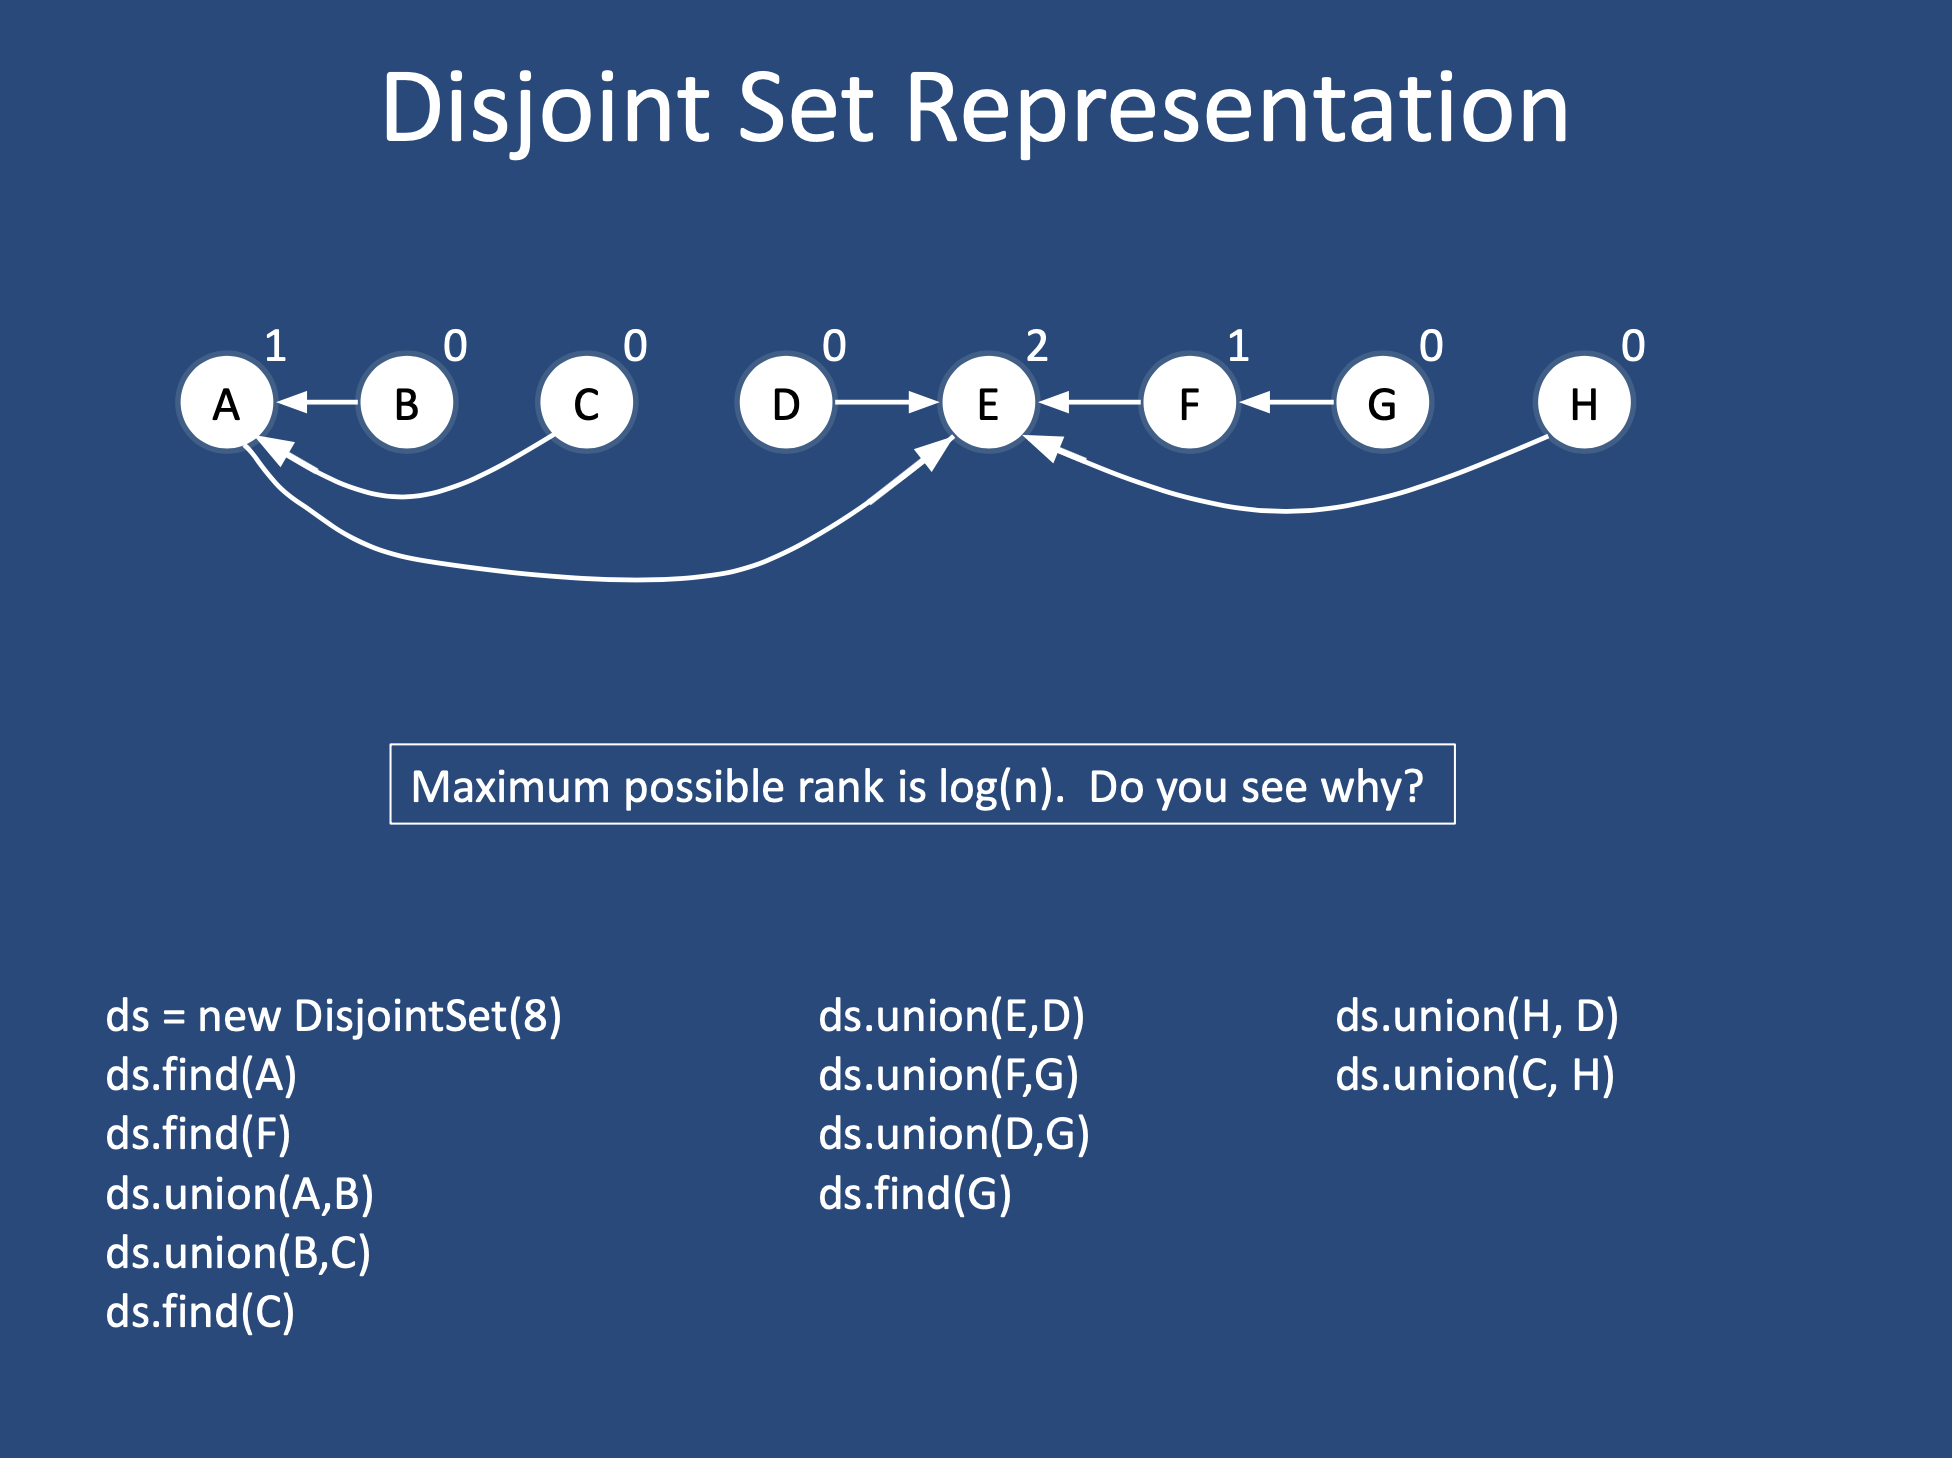
\includegraphics[width=\columnwidth]{disjoint_sets.png}
  \vskip 2pt
  \textit{Path Compression}: On each find operation, set the parent of the every vertex encountered to the found root to flatten tree.

  \vskip 15pt
  \textbf{Counting Sort} \\
  Counting sort is stable. Create a "count" array of size $\text{largest integer} + 1$. Iterate through the array, where $\text{count}[i] = $ number of integers that are $\leq i$. \\
  Iterate through the count array to fill in the result array. If $\text{count}[0] = 2$, then $\text{result}[0] = \text{result}[1] = 0$. If $\text{count}[1] = 3$, then index 0, 1, and 2 should be $\leq 1$. As index 0 and 1 are filled, then index 2 should be $1$.
  \begin{lstlisting}
for (i = data.length-1; i >= 0; i--) 
  index = --count[data[i]]
  newdata[index] = data[i]
  \end{lstlisting}
  Takes $O(\text{size of array} + \text{largest integer})$ time as it is not comparison based sorting.

  \vskip 7pt
  \hrule
  \vskip 7pt

  \textbf{Radix Sort} \\
  As counting sort is stable, make multiple passes of counting sorting but sort on a different byte each time. Therefore, radix sort is $O(kn)$ with $k$ byte integers.

  \vskip 7pt
  \hrule
  \vskip 7pt

  \textbf{RSA Algorithm} \\
  1. Select two distinct primes ($p$ and $q$). \\
  2. Let $N = pq$, the modulus. \\
  3. Let $\phi = (p - 1)(q - 1)$. \\
  4. Let $e > 1$ be a small integer where $gcd(e, \phi) = 1$. This is the public exponent. \\
  5. Choose $d$ such that $ed \equiv 1\mod\phi$. This is the private exponent. \\
  6. Let $P = (e, N)$, the public key. Let $S = (d, N)$, the private key. \\
  7. Encrypt $x$ by computing $x^e \mod N$. \\
  8. Decrypt $y$ by computing $y^d \mod N$.

  \vskip 7pt
  \hrule
  \vskip 7pt

  \textbf{Primality} \\
  Can test if an integer $p$ is prime multiple ways. \\
  1. Use the AKS algorithm, which is $O(n^2)$. \\
  2. Use the probabilistic prime test using Fermat's Little Theorem: \\
  If $p$ is prime, then $\forall a$ where $1 \leq a < p$, $a^{p-1} \equiv 1 \mod p$. For non Carmichael numbers, $a$ will fool the test at most half the time. Run Fermat's little theorem multiple times to get statistical certainty that the number is prime. \\
  Lagrange's theorem says that as $\lim_{x \rightarrow \infty}$, number of primes is $\leq \frac{x}{x / \ln x}$. Helps estimate probability a randomly chosen n-bit integer will be prime.

  \textbf{Electronic Commerce} \\
  Order of operations: \\
  1. Browser requests server’s signed certificate signed using its private key. \\
  2. Browser verifies certificate by decrypting using CA’s (certificate authority) public key (comes pre-installed on machines). \\
  3. Browser generates AES key, encrypts it with the server’s public key (contained in certificate) and sends it to the server. \\
  4. Server decrypts the AES key using its private key. \\
  5. Communication with symmetric AES key between client and server continues. \\
  Use AES after RSA because RSA encryption/decryption is slow.

  \vskip 7pt
  \hrule
  \vskip 7pt

  \textbf{Dynamic Programming} \\
  Store the results of repeated recursive calls to speed up programs. Program exhibits the optimal substructure property but there does not exist a greedy solution. \\
  1. Memoization: store parameters and result in a dictionary or array. This tends to be easier and will be faster if few subproblems need to be solved. \\
  2. Table iteration: if all subproblems must be solved, table iteration is faster. \\
  Example:
  \begin{lstlisting}
if uncloseable == 0:
  return max(values[r][0] + maxValue(r + 1, 
    0, k - 1), values[r][0] + values[r][1] 
    + maxValue(r + 1, -1, k))
elif uncloseable == 1:
  ...
else:
  return max(values[r][0] + maxValue(r + 1, 
    0, k - 1), values[r][1] + maxValue(r + 1, 
    1, k - 1), values[r][0] + values[r][1] 
    + maxValue(r + 1, -1, k))
  \end{lstlisting}
  Solve for the smallest problems first, growing to the larger problems.
  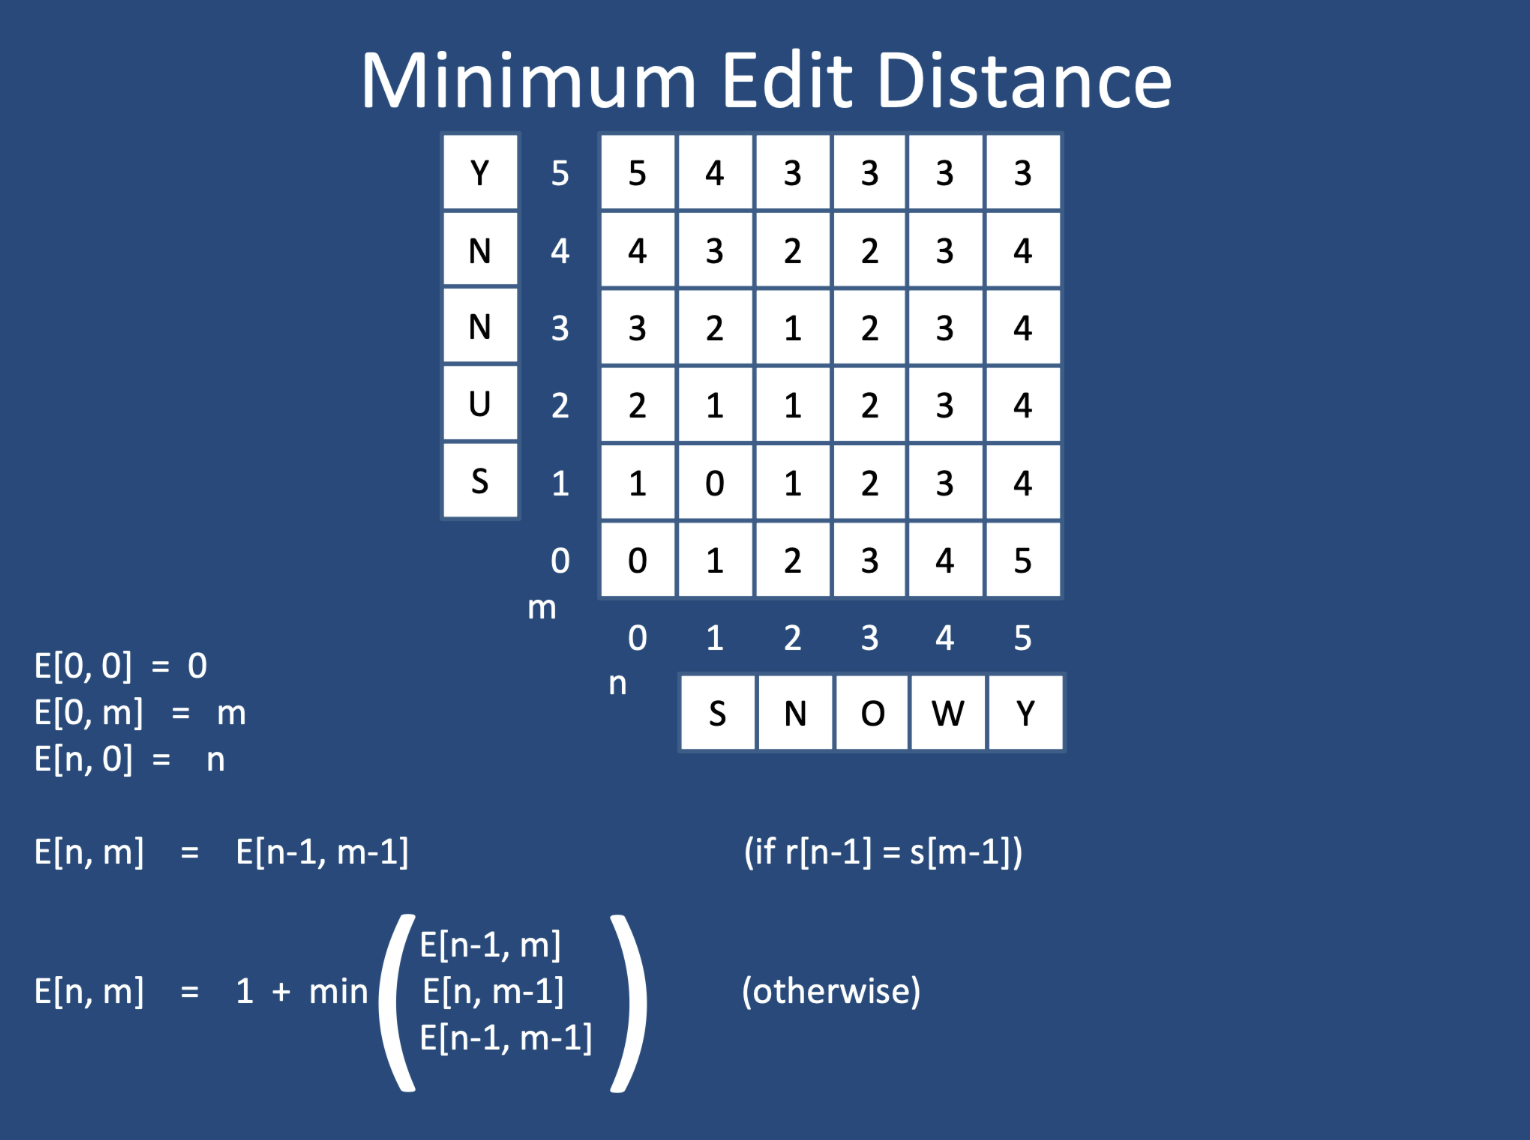
\includegraphics[width=\columnwidth]{minimum_edit.png}

  \textbf{Linear Programming} \\
  Solving optimization problems in which the constraints and the optimization criterion are linear inequalities. Example:
  \begin{lstlisting}
max: r + 1.5s;
s >= 0;
r >= 0;
s <= 0.5r;
r+s <= 3000;
  \end{lstlisting}

  The constraints give us a "feasible region". Find the maximum point in the feasible region that fulfills the objective function. If region is bounded, we will have an optimal solution. If unbounded, may or may not have optimal solution. Empty, no solution.

  \vskip 7pt
  \hrule
  \vskip 7pt

  \textbf{Duality} \\
  If a linear program has a bounded optimum, then so does its dual, and the two optimum values are the same. \\
  1. Primal:
  \begin{lstlisting}
max: A + B + C + D;

A = 0;
B <= A + 5;
B <= C + 1;
C <= A + 3;
C <= D + 4;
D <= B + 2; 
  \end{lstlisting}
  2. Multiply by new variables:
  \begin{lstlisting}
uA = 0
vB <= vA + 5v
wB <= wC + w
xC <= xA + 3x
yC <= yD + 4y
zD <= zB + 2z
  \end{lstlisting}
  3. Rearrange
  \begin{lstlisting}
uA = 0
vB - vA <= 5v
wB - wC <= w
xC - xA <= 3x
yC - yD <= 4y
zD - zB <= 2z
  \end{lstlisting}
  4. Add and collect terms:
  \begin{lstlisting}
(u-v-x)1A + (v+w-z)1B + (x+y-w)1C 
+ (z-y)1D <= 5v + w + 3x + 4y + 2z
  \end{lstlisting}
  5. Resulting dual program:
  \begin{lstlisting}
min:  5v + w + 3x + 4y + 2z

u-v-x >= 1; // 1 comes from 1A
v+w-z >= 1; // 1 comes from 1B
x+y-w >= 1; // 1 comes from 1C
z-y >= 1;   // 1 comes from 1D
v, w, x, y, z >= 0; 
  \end{lstlisting}

  \textbf{Decision, Search, Optimization} \\
  1. Decision: Is there a solution? \\
  2. Search: What is the solution? \\
  3. Optimization: What is the best solution?
  \vskip 1pt
  \textit{Decision to Search}: Take entire input space. Repeatedly remove elements from input space and check if valid solution. \\
  \textit{Search to Optimization}: Optimal solution must be between MIN and MAX of all possible inputs. Run binary search to find the optimal solution between MIN and MAX.

  \vskip 7pt
  \hrule
  \vskip 7pt

  \textbf{P and NP} \\
  $P$ is the set of all search problems that can be solved in polynomial time. \\
  $NP$ is the set of all search problems that can be verified in polynomial time. \\
  $NP$-complete is the set of the hardest problems in $NP$. All $NP$ problems must reduce to an $NP$-complete problem in polynomial time. Showing polynomial time algorithm for $NP$-complete problem gives polynomial time algorithm for all $NP$ problems. \\
  Examples are 3-SAT, TSP, Hamiltonian Path, Knapsack, Subset Sum, and Longest Path.
  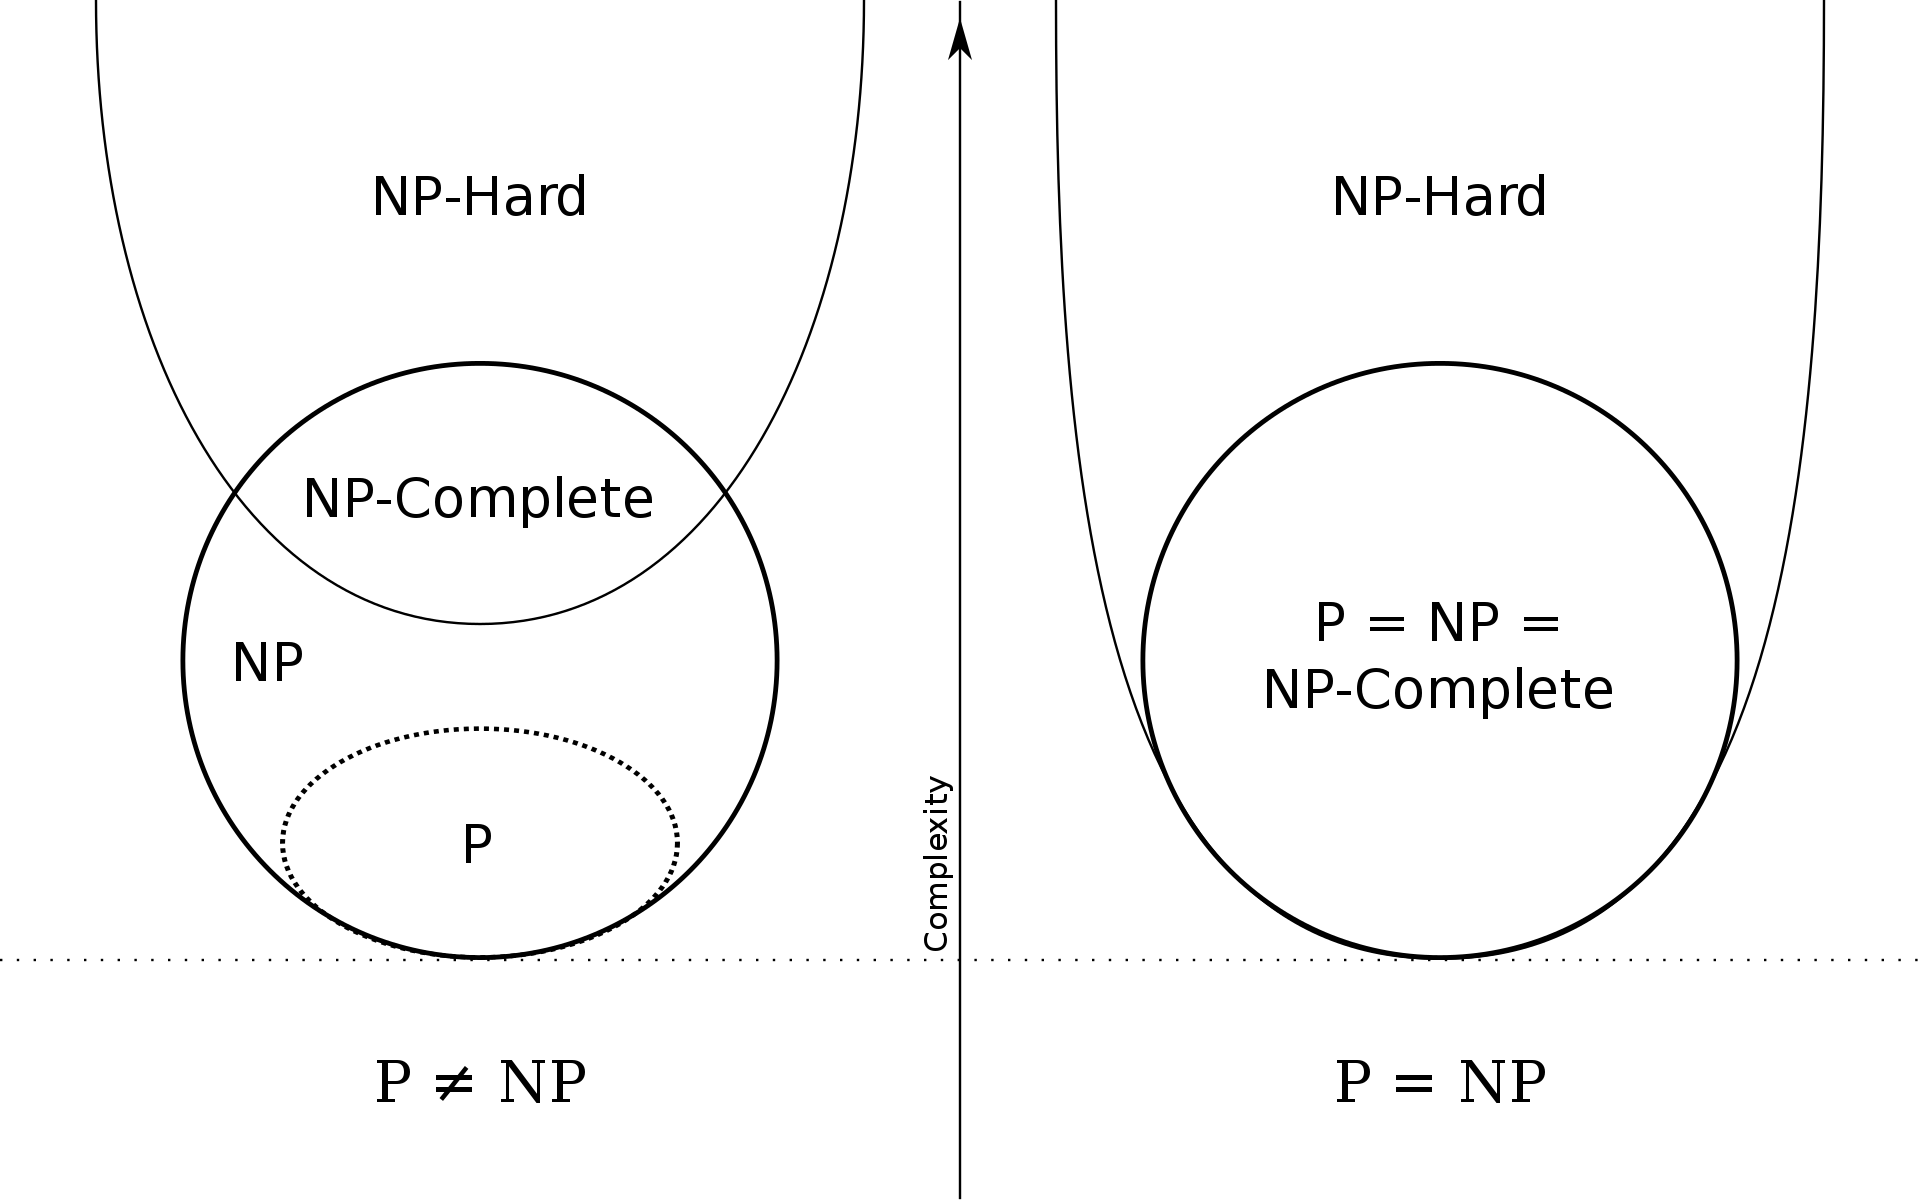
\includegraphics[width=\columnwidth]{pnp.png}
  To prove a problem $X$ is $NP$-complete, reduce a \textit{known} $NP$-complete problem to $X$ in polynomial time.

  \vskip 7pt
  \hrule
  \vskip 7pt

  \textbf{Reductions} \\
  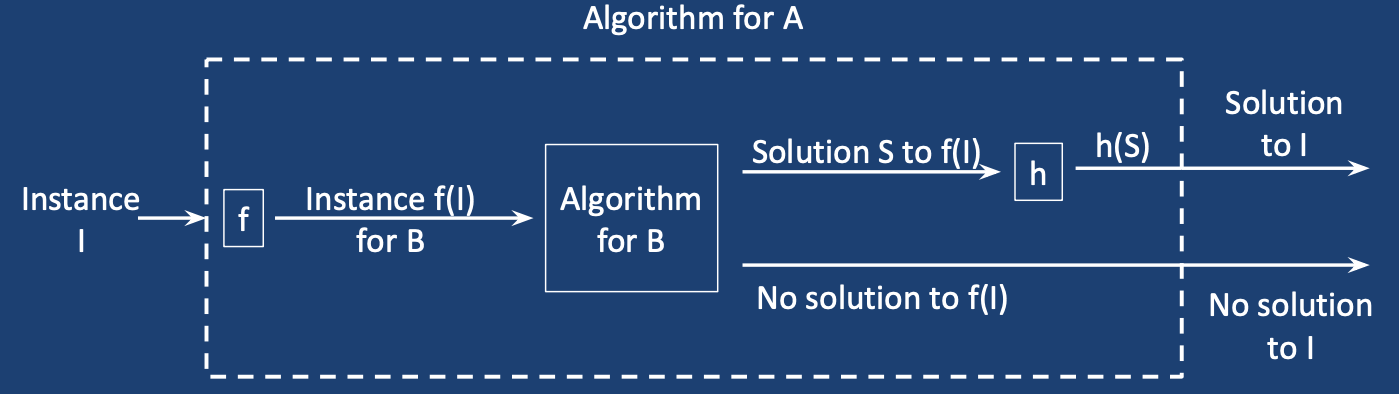
\includegraphics[width=\columnwidth]{reduction.png}
  Find function to transform input to $A$ to input of $B$. Run $B$. Transform output of $B$ to fit output of $A$. If these transformation functions run in polynomial time, this is a polynomial time reduction.\\
  Example: A finds largest element. B finds smallest element. Reducing A to B. Negate input to A, pass to B, then negate output of B.

  \textbf{Method Satisfiability} \\
  SAT was the first problem proven to be $NP$-complete. Take a function as an input, where the function returns true or false. Return false if the function can never be true or return some input that makes the given function return true. All other $NP$ problems reduce to SAT, therefore it is $NP$-complete. 

  \vskip 7pt
  \hrule
  \vskip 7pt

  \textbf{Unsolvable Problems} \\
  There are problems so difficult no algorithm has been found to ever solve them. Such as finding roots of Diophantine equations ($x^3yz + 2y^4z^2 - 7xy^tz = 6$) or the halting problem. These do not belong to $NP$.

  \vskip 7pt
  \hrule
  \vskip 7pt

  \textbf{Coping with NP Completeness} \\
  1. Special cases: efficient algorithms for special cases. Correct all the time, efficient most of the time. \\
  2. Backtracking (search problems): Enumerate the possibilities until you find a solution, but be clever about the order in which you consider the possibilities \\
  3. Branch and Bound (optimization problems): Sift through the possibilities looking for the best ones, but be clever about identifying fruitless possibilities as early as possible. Lower bound computation must be fast, should take constant time.\\
  4. Approximation: efficient algorithms that give approximate answers. Approximately correct, efficient all of the time. \\
  Examples: TSP with triangle inequality. Independent set problem when the graph is a tree. \\
  The approximation ratio $\alpha_A$ for approximation algorithm $A$ is the larger of
  \[
    \max_{instances\ i} A(I) / Opt(I)
  \]
  \[
    \max_{instances\ i} Opt(I) / A(I)
  \]
  Where $Opt$ is the optimal solution. The best ratio is 1.

  For TSP, there is no finite ratio. For TSP with triangle inequality, fixed lower bound $> 1$. For set cover, ratio is close to $\log N$. For knapsack, ratio is arbitrarily close to 1 by scaling everything down.

  Approximation algorithms do not prove anything about NP completeness.





\end{multicols*}
\end{document}